\subsection{Overview of the User Interface}
According to Software Requirement Specification document(SRS), this embedded software system shall provide the graphic user interface for user to interact with the EV3 robot via graphic icons, file input and output. The below is the list of functionalities of GUI mentioned in SRS:
\begin{itemize}
	\item The user is able to control the robot manually.
	\item The user is able to command the robot to move to specific point in the map under manual mode.
	\item The user is able to switch the current mode (Navigation and Manual modes) of the robot.
	\item The user is able to see the obstacles, line track displaced on the map.
	\item The user is able to trace the robot's current position.
	\item The user is able to see the detailed system log including software and hardware of the robot.
	\item The user is able to import and export xml file to define and retrieve the map information.
\end{itemize}
\subsection{Deatailed Design of the User Interface}
\subsubsection{GUI's screen image}
Fig.5 shows the screen image of GUI for end user perspective. The GUI supports mouse and keyboard devices. Each device is linked to GUI via action listeners established by GUI. When the GUI is created, there are multiply listeners created to listen the events from input devices. The detail actions will be discussed in section 6.2.2  
\begin{figure}[H]
	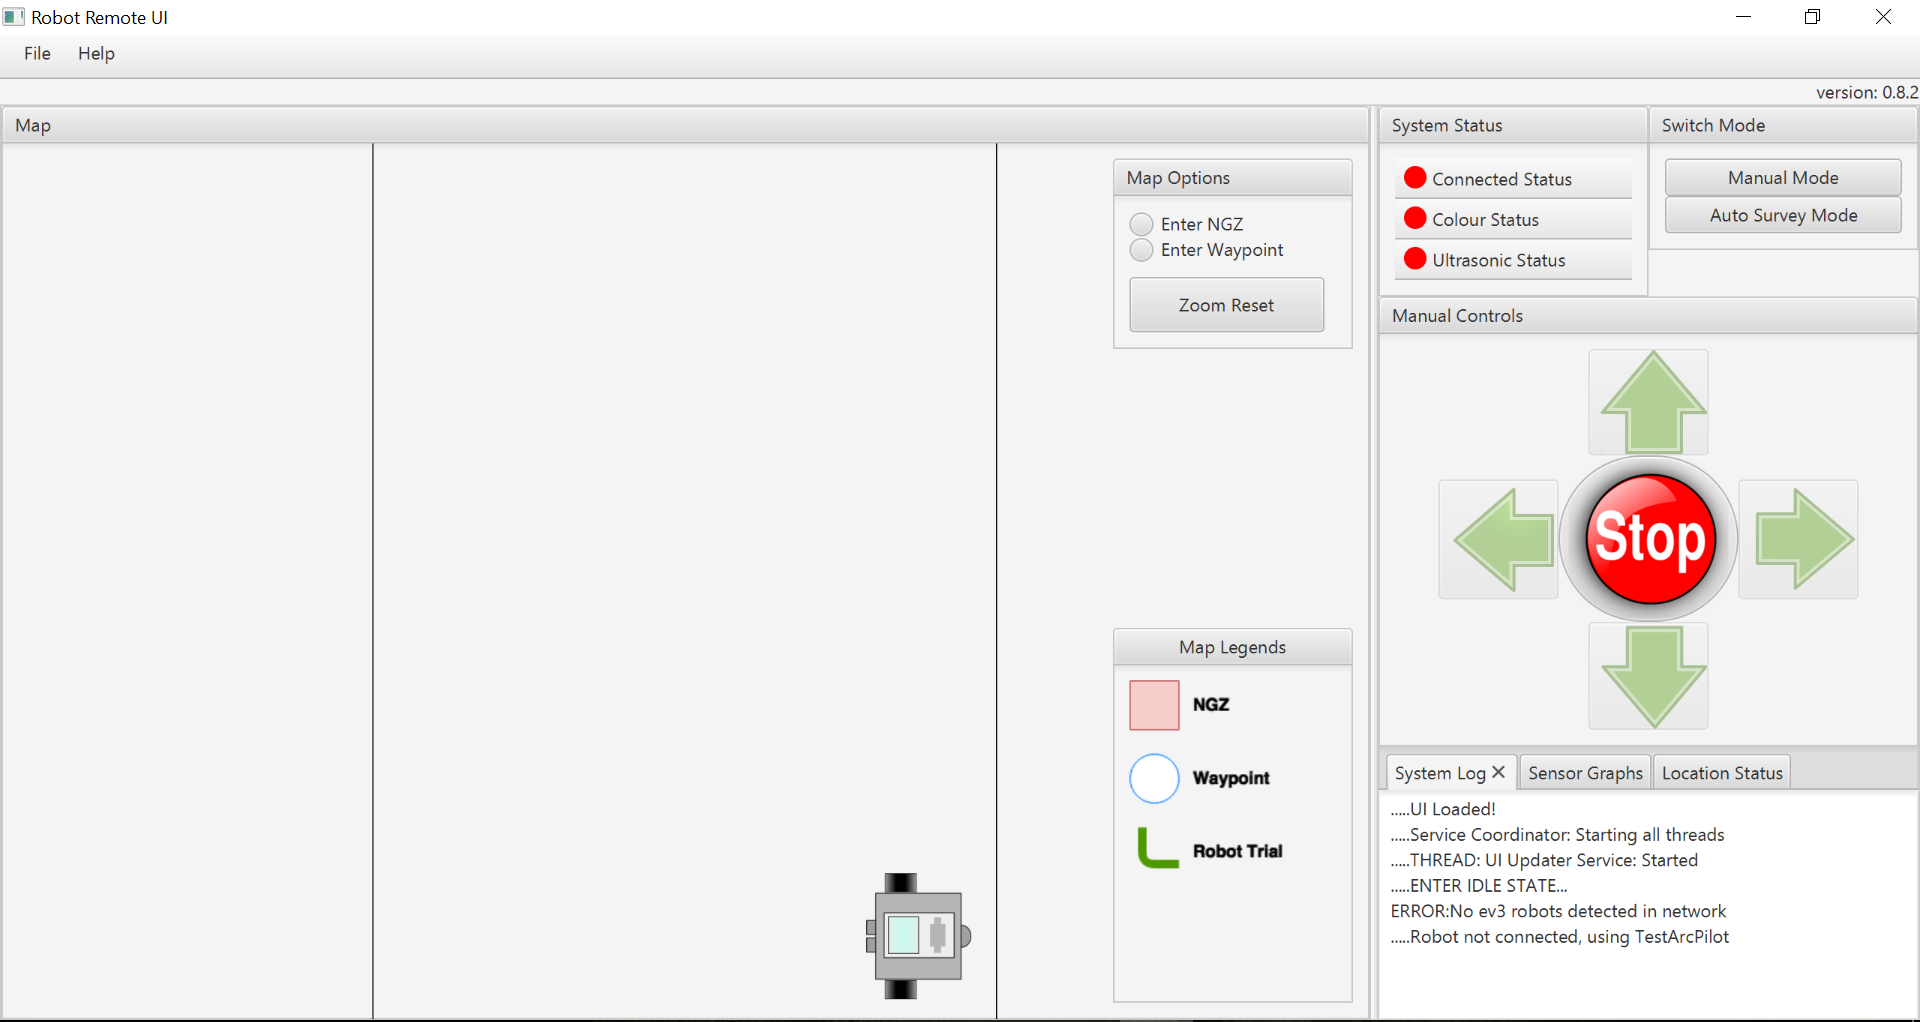
\includegraphics[width=\linewidth]{GUI.PNG}  % created using www.draw.io
	\caption{Graphic User Interface}
	\label{fig:Graphic User Interface}				
\end{figure}
\subsubsection{Screen Objects and Actions}
The GUI is divided into four main parts and listed in Table 1. Each part of GUI consists of mulitply panels.

\begin{table}[]
	\centering
	\caption{GUI Features}
	\label{GUI Features}
	\begin{tabular}{|l|l|l|}
		\hline
		Name             & Component & Related Features                       \\ \hline
		Mannual Control &           & UR13, UR14, FR008, FR009, FR010        \\ \hline
		Map area         &           & UR12, UR15, FR001, FR002, FR006, FR012 \\ \hline
		System status    &           & FR015                                  \\ \hline
		System log       &           & EM001                                  \\ \hline
	\end{tabular}
\end{table}

\begin{itemize}
	\item \textbf{1. Mannual Control}\\
	Supporting input devices: Keyboard and Mouse\\
	Mannual Control has two listeners for listen the event and determine the actions. One listener is for the event coming from mouse device. The another is for the event coming from keybroad. Fig.6 is the manual control panel
	\item  \textbf{Listener for listening mouse and keyboard event}\\
	The user can use their mouse to click the graphic icons showing on the Mannual Control panel to control the robot. Also, the user can use keyboard to fire the event to GUI to control the robot instead. Each button and keyboard listeners have different method to control the robot. For example, if the user click the stop button, the method called onClickStop() will be called and stop the robot movement. The list of methods called by listeners is shown on Table 2.
		
\begin{figure}[H]
	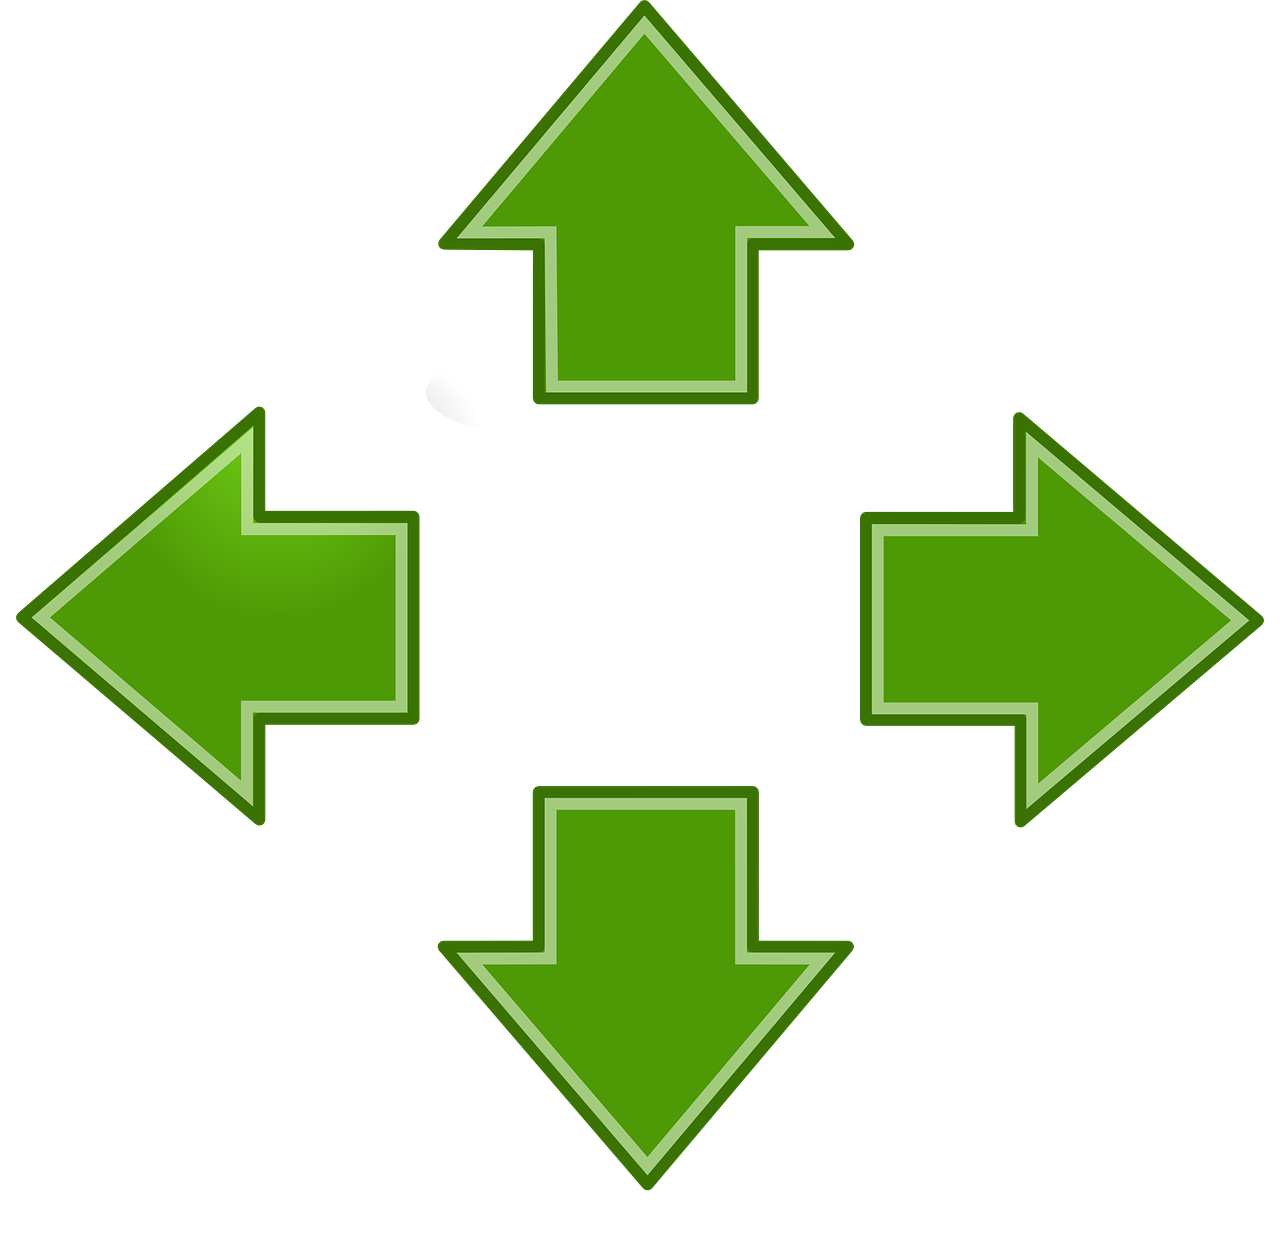
\includegraphics[width=\linewidth]{Control.PNG}  % created using www.draw.io
	\caption{Mannual control}
	\label{fig:Mannual controller}				
\end{figure}

\begin{table}[]
	\centering
	\caption{Method called for Manual Control}
	\label{Method called for Manual Control}
	\begin{tabular}{|l|l|l|l|}
		\hline
		\textbf{Method Name}            & \textbf{Graphic Buttons} & \textbf{KeyBoard Keys} & \textbf{Action} \\ \hline
		\textbf{onClickForward}  & \parbox[c]{1em}{
\includegraphics[width=15mm]{Up.png}} & W & Moving Forward  \\ \hline
		\textbf{onClickBackward} & \parbox[c]{1em}{
\includegraphics[width=15mm]{Down.png}} & S & Moving Backward \\ \hline
		\textbf{onClickLeft}     & \parbox[c]{1em}{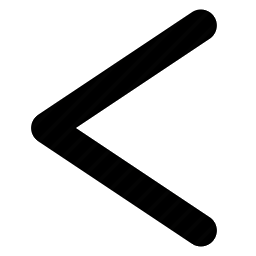
\includegraphics[width=15mm]{Left.png}} & A & Turn Left       \\ \hline
		\textbf{onClickRight}    & \parbox[c]{1em}{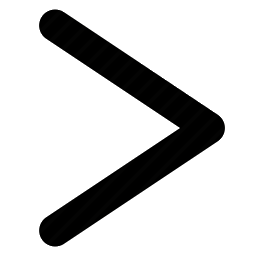
\includegraphics[width=15mm]{Right.png}} & D & Turn Right      \\ \hline
		\textbf{onClickStop}     & \parbox[c]{1em}{
\includegraphics[width=15mm]{Stop.png}}  & Q & Stop the robot  \\ \hline
	\end{tabular}
\end{table}
\end{itemize}

\begin{itemize}
	\item \textbf{2. Map Area}\\
	Supporting input devices: Mouse\\
	The Map showing on Figure 6 is to display the area where the robot need to be explored. The user can select the NGZ area in the map and change size of the map. Also, the detected obstacles, NGZ area and track line will also be displayed in the map. The user can check the map legend to see what it looks in the map. Mouse listener will be created in the map to listen the event from the mouse. The list of methods called by listeners is shown on Table 3.

\begin{table}[]
	\centering
	\caption{Methods called by map listeners}
	\label{Methods called by map listeners}
	\begin{tabular}{|l|l|}
		\hline
		\textbf{Name}             & Mouse Action and Action                                                                                                                                                                                                                             \\ \hline
		\textbf{onClickZoomReset} & Click on the reset button                                                                                                                                                                                                                           \\ \hline
		\textbf{onClickMap}       & \begin{tabular}[c]{@{}l@{}}If the user ticks the "Enter way point" box,\\ then the user clicks on the map, the robot will go to that point.\\ If the user ticks the "Ener NGX" box,\\ then the user can select the NGZ area on the map\end{tabular} \\ \hline
		\textbf{onDragMap}        & Determine the map action, the user do not need to concern this method                                                                                                                                                                               \\ \hline
	\end{tabular}
\end{table}
\end{itemize}

	